\documentclass[11pt]{article}


\setlength{\parindent}{0pt}
\usepackage{xltxtra}
\usepackage{hyperref}
\hypersetup{hidelinks}
\usepackage{url}
\urlstyle{tt}
\usepackage{xcolor}
\definecolor{CVBlue}{RGB}{23,110,191}
\usepackage{calc}
\usepackage{graphicx}
\usepackage{tikz}
\usetikzlibrary{calc}
\usepackage{fontspec}
\usepackage{xeCJK}
\usepackage{enumitem}
\CJKsetecglue{} %% 取消中文与数字之间的间隙


%% 主文档字体设置
\setmainfont[
    Path = fonts/Main/,
    Extension = .otf,
    BoldFont = texgyretermes-bold.otf, % 加粗字体
]{texgyretermes-regular.otf} % 正文字体

% 中文字体设置
\setCJKmainfont[
    Path = fonts/hansans/,
    Extension = .ttf,
    BoldFont = NotoSansSC-Bold.ttf, % 加粗字体
]{NotoSansSC-Regular.otf} % 正文字体


\usepackage{relsize}
\usepackage{xspace}

% 使用 fontawesome（部分图标）
\usepackage{fontawesome} 

% A4纸，上下左右边距
\usepackage[
    a4paper,
    left=1.2cm,
    right=1.2cm,
    top=1.5cm,
    bottom=1cm,
    nohead
]{geometry}

\renewcommand{\baselinestretch}{1.5} % 行间距设为1.5

\usepackage{titlesec}
\usepackage{enumitem}
\setlist{noitemsep} % 取消列表项间的额外间距
%\setlist{nosep} % 取消所有垂直间距
\setlist[itemize]{topsep=0.25em, leftmargin=*}
\setlist[enumerate]{topsep=0.25em, leftmargin=*}

% --- 用于控制【不同项目之间】的垂直距离 ---
\newlength{\interProjectSpacing}
\setlength{\interProjectSpacing}{0.9em} % <--- 在此调整项目之间的距离
\newcommand{\projectsep}{\vspace{\interProjectSpacing}}

% --- 用于控制【项目标题】与下方【项目描述】的距离 ---
\newlength{\intraProjectTitleSep}
\setlength{\intraProjectTitleSep}{0.4em} % <--- 在此调整标题和描述的距离
\newcommand{\titlebreak}{\\[\intraProjectTitleSep]}

% --- 用于控制【项目描述】与下方【要点列表】的距离 ---
\newlength{\intraProjectListTopSep}
\setlength{\intraProjectListTopSep}{0.2em} % <--- 在此调整描述和列表的距离

% =======================================================================


\titleformat{\section}         % 定制 \section 命令 
{\large\bfseries\raggedright} % 将 section 标题设置为大号、粗体且左对齐
{}{0em}                      % 可用于为所有 section 添加前缀（如“章节...”）
{}                           % 可用于在标题前插入代码
[{\color{CVBlue}\titlerule}]  % 在标题后插入一条横线
\titlespacing*{\section}{0cm}{*1.6}{*1.2}



\begin{document}
\pagenumbering{gobble}

  %%%% 利用tikz来定位学校Logo，这里只在第一页显示
  \begin{tikzpicture}[remember picture, overlay] 
    \node[anchor = north west] at ($(current page.north west)+(0.5cm,+1.0cm)$) {
\includegraphics[height=6cm]{bjut.png}};
  \end{tikzpicture}%

\begin{center}
    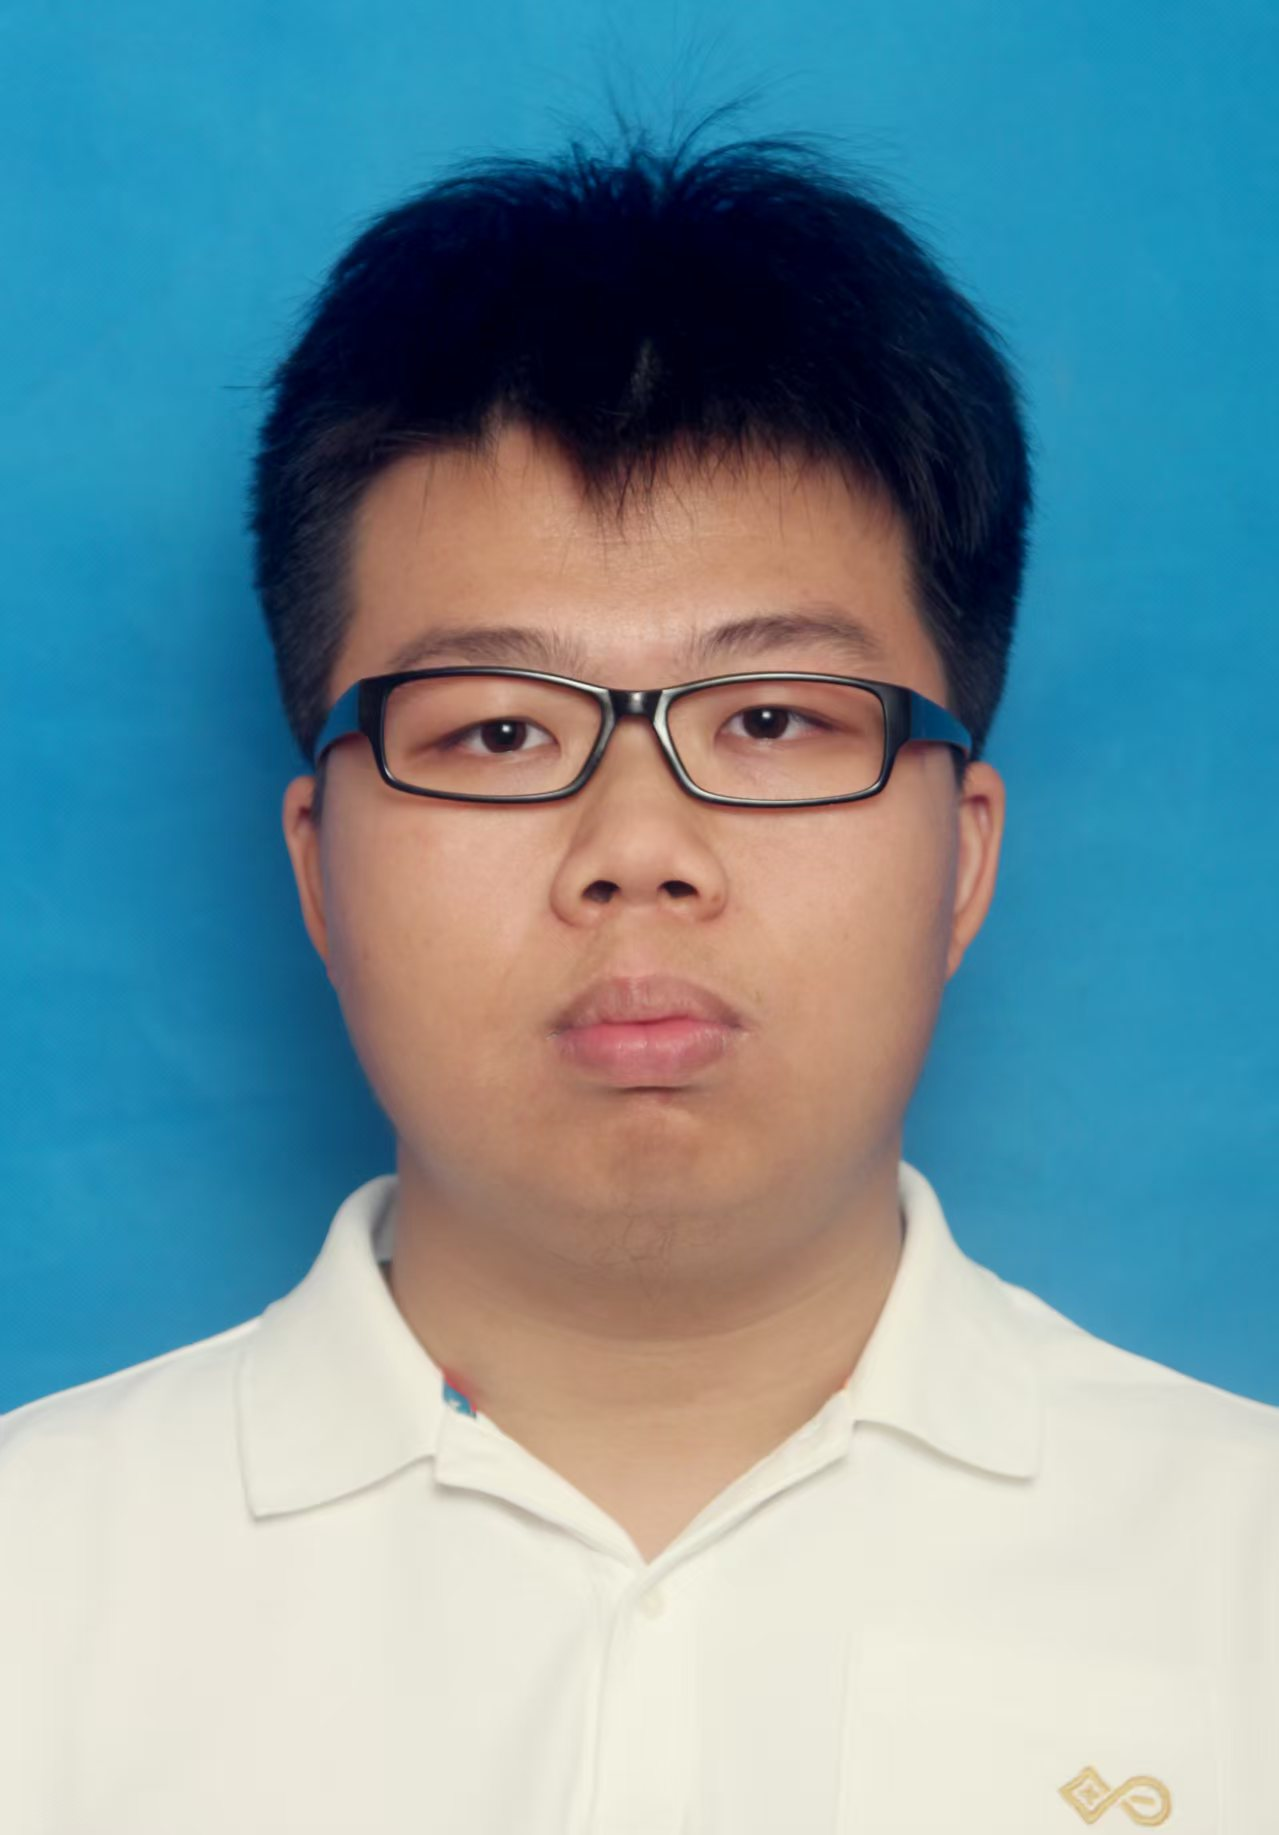
\includegraphics[width=3cm]{证件照.jpg}
\end{center}
\centerline{\LARGE\bfseries{曾爱文}} 

\centerline{\normalsize{\faPhone\ 185-1337-1062 \quad \faEnvelopeO\ \href{mailto:zaw23073109@emails.bjut.edu.cn}{zaw23073109@emails.bjut.edu.cn}}} 
  
\centerline{\normalsize{\faGithubSquare\ \href{https://github.com/MolexZzz}{https://github.com/MolexZzz}}} 
    
\section{\makebox[\widthof{\faGraduationCap}][c]{\color{CVBlue}\faGraduationCap}\ 教育背景}    
\textbf{北京工业大学} \hfill 2023.9 -- 至今\\[0.5em] % 标题和正文间加一点距离
计算机科学与技术\quad 大三 \\
加权平均分：94.04/100\quad 排名：3/61       
\begin{itemize}[nosep]
    \item 相关课程：《高等数学》(100)、《线性代数》(99)、《概率论与数理统计》(98)、集合与图论(96)、《代数与逻辑》(96)、《数据结构与算法》(92)、《计算机组成原理》(97)、《计算机系统结构》(100)、《操作系统原理》(85)、《计算机网络》(92)、《数据库原理》(89)、《人工智能导论》(94)、《模式识别》(98)
\end{itemize}

\section{\makebox[\widthof{\faUsers}][c]{\color{CVBlue}\faUsers}\ 项目学习经历} 

    % --- 第一个项目 ---
    \textbf{多模态混合向量检索系统} \hfill 2025.01 -- 至今 \titlebreak
    \textbf{指导老师：}中国科学院软件研究所许利杰研究员、秦政助理研究员
    项目描述：针对多模态数据的向量检索场景，设计并实现了一套融合语义与视觉特征的混合向量检索系统。核心创新包括提出\textbf{HDMG(分层动态度量图)}索引结构用于加速混合查询，以及实现跨多个向量数据库的性能对标评测框架。
    \begin{itemize}[nosep, topsep=\intraProjectListTopSep]
        \item \textbf{混合查询引擎}：设计了融合\textbf{语义向量(key向量)}与\textbf{视觉向量(图像embedding)}的混合查询方案，通过可调权重$\beta$平衡两个模态，实现细粒度检索意图控制。
        \item \textbf{HDMG图索引}：提出并实现了分层动态度量图结构，采用\textbf{embedding边}(向量距离KNN)与\textbf{semantic边}(语义相似度)双连通设计，将混合查询复杂度从O(N)降至O(log N)。
        \item \textbf{多数据集与多向量库对标测试}：拓展testbench覆盖\textbf{Caltech-101}(图像)、\textbf{20Newsgroups}(文本)等多个数据集，集成\textbf{Milvus、Qdrant、Chroma}三大向量数据库进行横向性能对比，通过大规模recall实验验证HDMG的加速效果。
        \item \textbf{数据集管理与自动聚类}：实现了向量组的参数化自动聚类(参数$\alpha$控制粒度)，支持向量序列追踪与上下文关系管理，确保数据集规模的有效扩展。
    \end{itemize}
    % 使用 \projectsep 命令来分隔两个项目
    \projectsep

    % --- 第二个项目 ---
    \textbf{基于X语言到仓颉语言的代码转化方案调研 (研究学习)} \hfill 2025.01 -- 2025.02 \titlebreak
    \textbf{指导老师：}中国科学院软件研究所许利杰研究员、秦政助理研究员
    项目描述：针对鸿蒙生态下海量遗留资产（Java/C++等）向原生\textbf{仓颉(Cangjie)}语言迁移的痛点，系统调研了软工顶会(FSE, TSE等)的\textbf{项目级代码转换}前沿技术，并撰写基于X语言到仓颉语言的代码转化方案调研PPT。
    \begin{itemize}
        \item \textbf{核心方法论与痛点破局}：对比了基于规则(如J2CJ)与传统序列模型的局限性，明确了\textbf{LLM+神经符号}的技术路线。针对仓颉作为低资源语言带来的“大模型幻觉”问题，总结了\textbf{骨架引导 (Skeleton-Guided)}、\textbf{逆拓扑排序调用}以及基于\textbf{RAG}的API知识注入等核心缓解策略。
        \item \textbf{评估基准与验证机制}：梳理了从小片段到\textbf{仓库级 (Repo-Level)}的评测基准演进 (如RepoTransBench, TransRepo)。深入探究了无需人工重写测试用例的\textbf{跨语言隔离测试 (In-Isolation Validation)}，以及利用\textbf{编译器反馈机制 (Compiler-Feedback)}强化模型翻译能力的闭环验证方案。
        \item \textbf{智能化软件工程(AI4SE)认知深化}：通过对大模型代码幻觉、跨文件循环依赖、低资源语言知识注入等共性问题的深度剖析，建立了对\textbf{智能化软件工程 (AI4SE)}的系统性认识。理清了从“代码片段翻译”到“真实工程迁移”的巨大技术鸿沟，极大拓宽了自身的科研视野与学术品味。
    \end{itemize}
    \projectsep

    % --- 第三个项目 ---
    \textbf{缓存替换算法性能分析与比较} \hfill 2025.02 -- 2025.06 \titlebreak
    \textbf{项目导师：}北京工业大学计算机学院王茜副教授
    项目描述：该项目旨在探究多种基于学习类的缓存替换算法在不同访问模式下的性能表现。
    \begin{itemize}[nosep, topsep=\intraProjectListTopSep]
        \item 搭建\textbf{libCacheSim}实验环境，配置并运行测试程序，评估不同算法在指定数据集上的性能。
        \item 使用\textbf{Python}脚本对实验产生的原始数据进行处理与聚合，提取\textbf{命中率、替换次数}等关键性能指标。
        \item 利用\textbf{Matplotlib}等数据可视化库，将各项性能指标进行图表化展示，直观比较各算法优劣，并通过分析潜在访问模式变化，提出算法改进建议。
    \end{itemize}
    
\section{\makebox[\widthof{\faCogs}][c]{\color{CVBlue}\faCogs}\ 专业技能}
\begin{itemize}[nosep]
    \item 掌握 C/C++、Python、Java
    \item 熟悉常用的数据结构与算法
    \item 掌握基本的传统机器学习方法
    \item 能在 Linux 环境下进行开发
    \item 熟练使用 Git 进行项目管理
\end{itemize}
\section{\makebox[\widthof{\faGraduationCap}][c]{\color{CVBlue}\faList}\ 获奖情况}
\begin{itemize}[nosep]
    \item 全国大学生数学竞赛北京赛区（非数学A类）三等奖 \hfill 2024.12
    \item 中国机器人及人工智能大赛百度Apollo（北京赛区）三等奖 \hfill 2025.08
    \item 中国机器人及人工智能大赛simuro足球（北京赛区）三等奖 \hfill 2025.08
    \item 北京工业大学2023-2024学年度学习优秀奖 \hfill 2024.09
    \item 北京工业大学2024-2025学年度学习优秀奖 \hfill 2025.09
\end{itemize}
    
\section{\makebox[\widthof{\faInfo}][c]{\color{CVBlue}\faInfo}\ 其他}
\begin{itemize}[parsep=0.5ex]
    \item \textbf{GitHub：} \href{https://github.com/MolexZzz}{https://github.com/MolexZzz} 
    \item \textbf{英语水平：} CET-4：554, CET-6：495
\end{itemize}
\end{document}
